


\tikzset{every picture/.style={line width=0.75pt}} %set default line width to 0.75pt        

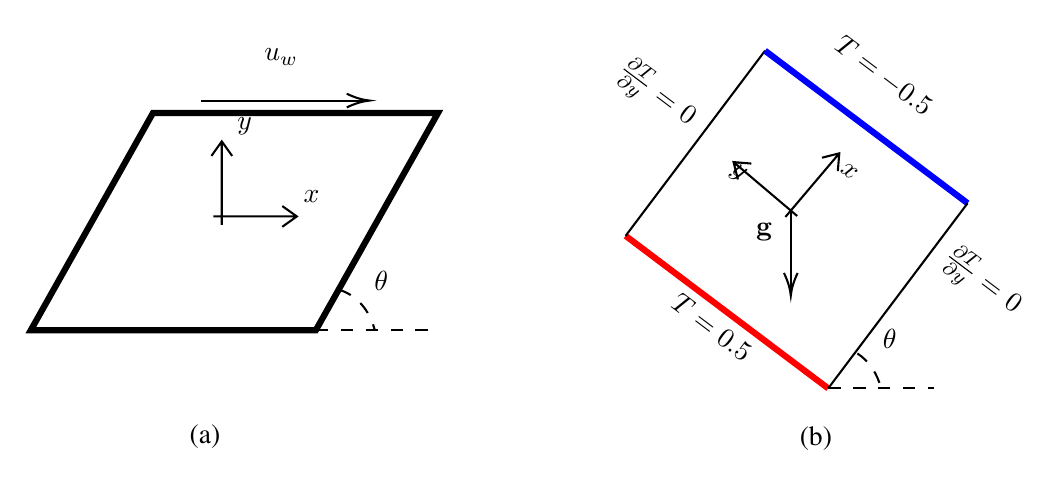
\begin{tikzpicture}[x=0.75pt,y=0.75pt,yscale=-1,xscale=1]
%uncomment if require: \path (0,300); %set diagram left start at 0, and has height of 300

%Shape: Parallelogram [id:dp9047639156855234] 
\draw  [line width=2.25]  (158.85,54.33) -- (296.17,54.33) -- (237.32,159) -- (100,159) -- cycle ;
%Straight Lines [id:da022102604490445987] 
\draw  [dash pattern={on 4.5pt off 4.5pt}]  (237.32,159) -- (294.17,159) ;
%Shape: Arc [id:dp3625941908227275] 
\draw  [draw opacity=0][dash pattern={on 4.5pt off 4.5pt}][line width=0.75]  (248.73,139.51) .. controls (249.54,139.77) and (250.34,140.08) .. (251.13,140.43) .. controls (258.56,143.77) and (263.59,150.61) .. (265.74,159) -- (235.33,175.6) -- cycle ; \draw  [dash pattern={on 4.5pt off 4.5pt}][line width=0.75]  (248.73,139.51) .. controls (249.54,139.77) and (250.34,140.08) .. (251.13,140.43) .. controls (258.56,143.77) and (263.59,150.61) .. (265.74,159) ;
%Straight Lines [id:da4686433463461326] 
\draw    (182.17,48.33) -- (261.17,48.33) ;
\draw [shift={(263.17,48.33)}, rotate = 180] [color={rgb, 255:red, 0; green, 0; blue, 0 }  ][line width=0.75]    (10.93,-3.29) .. controls (6.95,-1.4) and (3.31,-0.3) .. (0,0) .. controls (3.31,0.3) and (6.95,1.4) .. (10.93,3.29)   ;
%Straight Lines [id:da13054384610033587] 
\draw [color={rgb, 255:red, 255; green, 0; blue, 0 }  ,draw opacity=1 ][fill={rgb, 255:red, 255; green, 0; blue, 0 }  ,fill opacity=1 ][line width=2.25]    (386.58,113.51) -- (433.85,149.1) -- (441.84,155.12) -- (484.18,187) ;
%Straight Lines [id:da7865449518065537] 
\draw    (453.76,24.31) -- (386.58,113.51) ;
%Straight Lines [id:da6737074539920613] 
\draw [color={rgb, 255:red, 0; green, 0; blue, 255 }  ,draw opacity=1 ][fill={rgb, 255:red, 120; green, 75; blue, 37 }  ,fill opacity=1 ][line width=2.25]    (453.76,24.31) -- (551.35,97.79) ;
%Straight Lines [id:da9569221815502367] 
\draw    (484.18,187) -- (551.35,97.79) ;
%Shape: Axis 2D [id:dp8627886510879132] 
\draw  (188,104.15) -- (228.17,104.15)(192.02,68) -- (192.02,108.17) (221.17,99.15) -- (228.17,104.15) -- (221.17,109.15) (187.02,75) -- (192.02,68) -- (197.02,75)  ;
%Straight Lines [id:da0904797526413792] 
\draw    (466.17,101.33) -- (466.17,140.33) ;
\draw [shift={(466.17,142.33)}, rotate = 270] [color={rgb, 255:red, 0; green, 0; blue, 0 }  ][line width=0.75]    (10.93,-3.29) .. controls (6.95,-1.4) and (3.31,-0.3) .. (0,0) .. controls (3.31,0.3) and (6.95,1.4) .. (10.93,3.29)   ;
%Shape: Axis 2D [id:dp20639716300089672] 
\draw  (463.57,104.4) -- (489.53,73.75)(438.58,77.97) -- (469.23,103.93) (481.19,75.86) -- (489.53,73.75) -- (488.82,82.32) (440.69,86.31) -- (438.58,77.97) -- (447.15,78.68)  ;
%Straight Lines [id:da47495207476294654] 
\draw  [dash pattern={on 4.5pt off 4.5pt}]  (484.18,187) -- (535.17,187) ;
%Shape: Arc [id:dp0636775684298887] 
\draw  [draw opacity=0][dash pattern={on 4.5pt off 4.5pt}][line width=0.75]  (498.26,170.18) .. controls (503.94,173.87) and (507.84,179.87) .. (509.67,187) -- (479.26,203.6) -- cycle ; \draw  [dash pattern={on 4.5pt off 4.5pt}][line width=0.75]  (498.26,170.18) .. controls (503.94,173.87) and (507.84,179.87) .. (509.67,187) ;

% Text Node
\draw (264,129) node [anchor=north west][inner sep=0.75pt]   [align=left] {$\displaystyle \theta $};
% Text Node
\draw (211,22) node [anchor=north west][inner sep=0.75pt]   [align=left] {$u_{w}$};
% Text Node
\draw (389.16,23.31) node [anchor=north west][inner sep=0.75pt]  [rotate=-36.98] [align=left] {$\frac{\partial T}{\partial y}$ = 0};
% Text Node
\draw (545.94,113.6) node [anchor=north west][inner sep=0.75pt]  [rotate=-36.98] [align=left] {$\frac{\partial T}{\partial y}$ = 0};
% Text Node
\draw (412.94,138.36) node [anchor=north west][inner sep=0.75pt]  [rotate=-36.98] [align=left] {$T=0.5$};
% Text Node
\draw (491.78,13.71) node [anchor=north west][inner sep=0.75pt]  [rotate=-36.98] [align=left] {$T=-0.5$};
% Text Node
\draw (230,90) node [anchor=north west][inner sep=0.75pt]   [align=left] {$\displaystyle x$};
% Text Node
\draw (198,55) node [anchor=north west][inner sep=0.75pt]   [align=left] {$\displaystyle y$};
% Text Node
\draw (448,106) node [anchor=north west][inner sep=0.75pt]   [align=left] {$\mathbf{g}$};
% Text Node
\draw (492.73,75.76) node [anchor=north west][inner sep=0.75pt]  [rotate=-36.55] [align=left] {$\displaystyle x$};
% Text Node
\draw (439.87,75.59) node [anchor=north west][inner sep=0.75pt]  [rotate=-36.55] [align=left] {$\displaystyle y$};
% Text Node
\draw (509,157) node [anchor=north west][inner sep=0.75pt]   [align=left] {$\displaystyle \theta $};
% Text Node
\draw (175,203) node [anchor=north west][inner sep=0.75pt]   [align=left] {{\fontfamily{ptm}\selectfont (a)}};
% Text Node
\draw (469,204) node [anchor=north west][inner sep=0.75pt]   [align=left] {{\fontfamily{ptm}\selectfont (b)}};


\end{tikzpicture}